\section{Terrain Classifier Creation (2 pages)}

We will train, test, and evaluate multiple neural networks in their ability to predict the
``correct'' safety mask of the landing sites in the synthetic data sets.
We will focus first on using U-nets to map from the input LIDAR or RGBD image
to the output mask, as they have been proven to be good classifiers in many different scenarios,
from terrain analysis, to tissue analysis, to road identification, etc.
We anticipate that the main challenge in this domain will not be
to train the networks, but rather to keep them small enough
so that they can execute quickly on embedded hardware.
Nevertheless, we will start by focusing strictly on maximizing the ability of the networks
to accurately predict the safety masks.

As an example of how this will work, we take an example from my project in RU's Deep Learning
course, wherein my group member and I used a Residual U-net to classify defects
in manufactured steel.
More than 17,000 images were labeled by hand, according to which of 4 defects they contained.
Figure \ref{figure:steel_defect_images} shows an example of the input data from this project,
where the yellow and blue outlines show the locations of different types of defect areas.

\begin{figure}
    \centering
    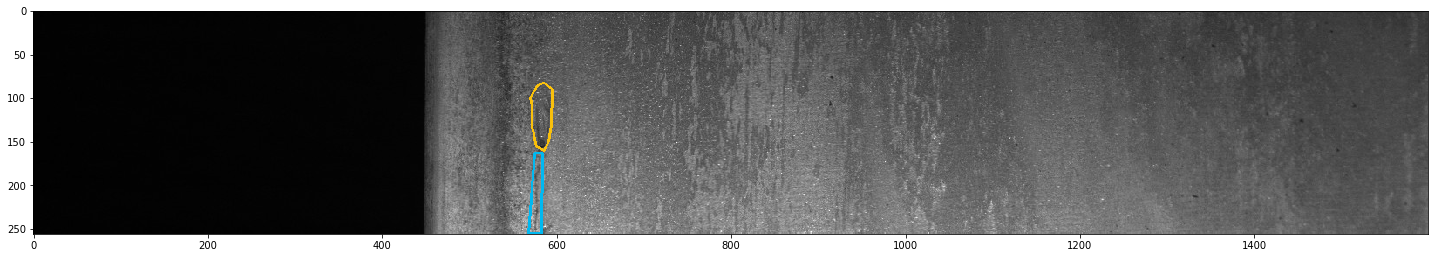
\includegraphics[width=\textwidth]{images/masked_image_1.png}
    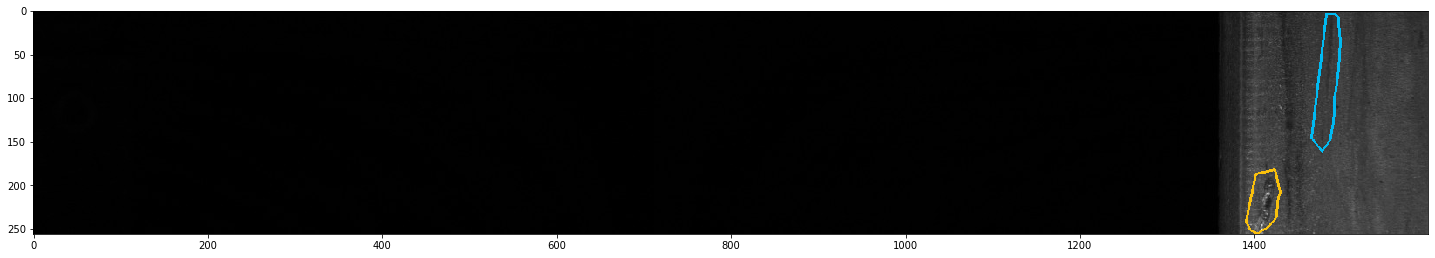
\includegraphics[width=\textwidth]{images/masked_image_2.png}
    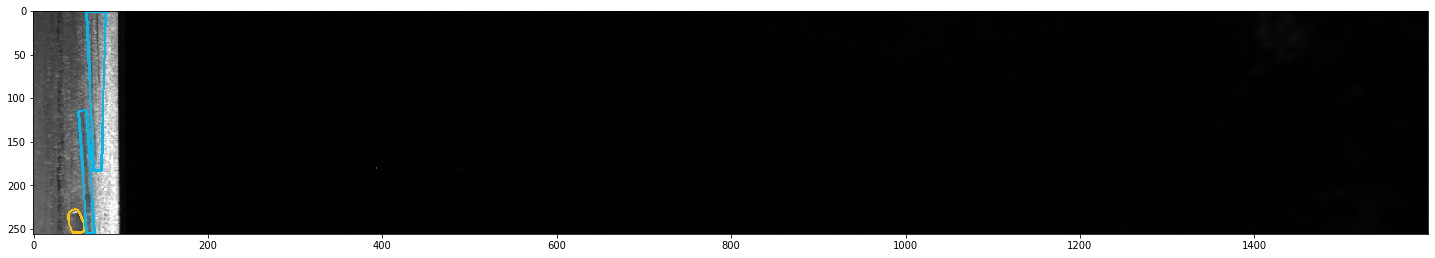
\includegraphics[width=\textwidth]{images/masked_image_3.png}
    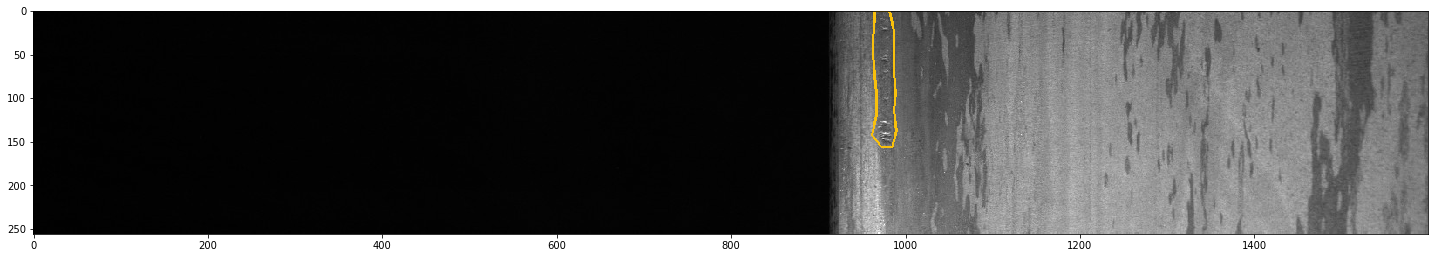
\includegraphics[width=\textwidth]{images/masked_image_4.png}
    \caption{Samples of typical steel defect images with their defect masks outlined.}
    \label{figure:steel_defect_images}
\end{figure}

This particular project was very time-limited, so the network trained for only 4 epochs,
but was able to achieve about 50\% prediction accuracy in that time,
and its output for an example image can be seen in Figure \ref{figure:example_steel_prediction}.
This project also gave some insight into accuracy metrics that can help bias the output
for/against false positives/negatives.
For example, in the case of the steel defect recognition, we used a Tversky metric to
reduce the amount of false negative defect classifications because a second step of the
process is for a human to manually examine the defect-classified steel before discarding it.
In this context it is better to make the network more ``cautious,'' in the hopes that
alerting the human to some false defects will mean that the network never incorrectly approves
defected steel for sale.
Conversely, in the case of autonomous drones,
we would like the networks to be conservative in their identification of safe landing sites,
so that they never direct the drone to land in unsafe landing sites, even though they may reject
some landing sites that are actually safe.
This is purely to give an intuition of the form of the problem we will use the classifiers to solve.

\begin{figure}
    \centering
    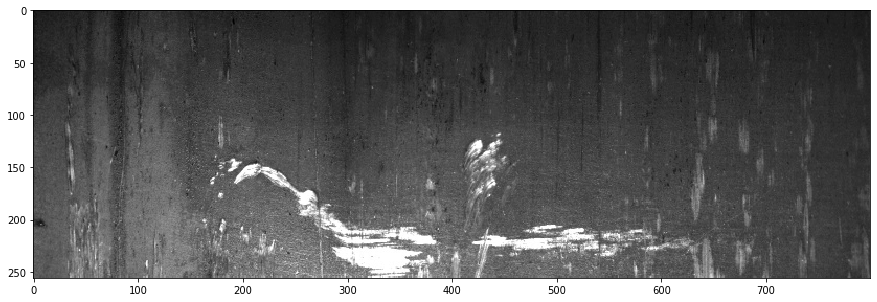
\includegraphics[width=\textwidth]{images/original_image.png}
    \subfloat[Defect 1 Mask]{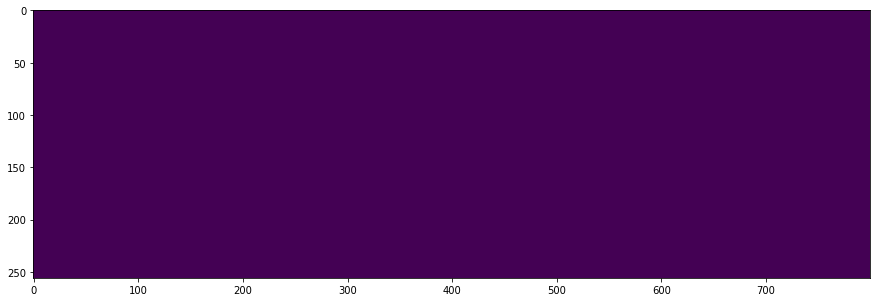
\includegraphics[width = 0.5\textwidth]{images/true_def0.png}}
    \subfloat[Defect 1 Prediction]{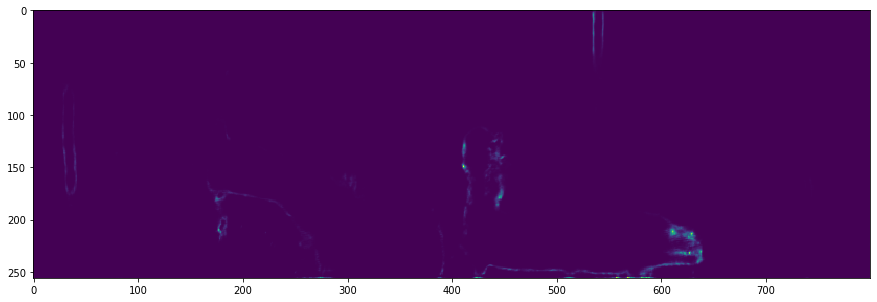
\includegraphics[width = 0.5\textwidth]{images/pred_def0.png}}\\
    \subfloat[Defect 2 Mask]{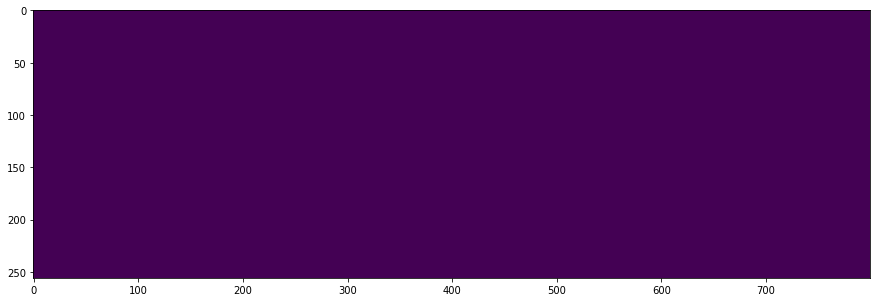
\includegraphics[width = 0.5\textwidth]{images/true_def1.png}}
    \subfloat[Defect 2 Prediction]{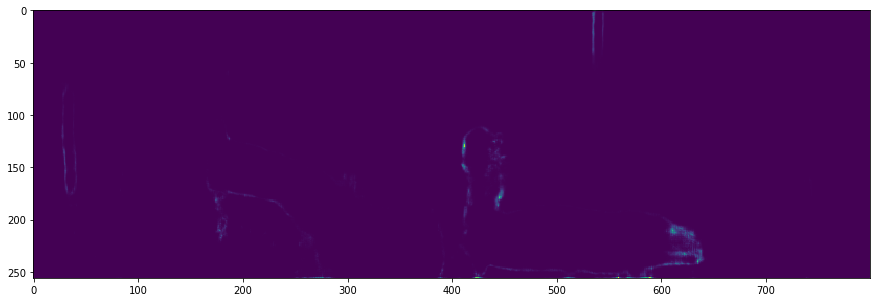
\includegraphics[width = 0.5\textwidth]{images/pred_def1.png}}\\
    \subfloat[Defect 3 Mask]{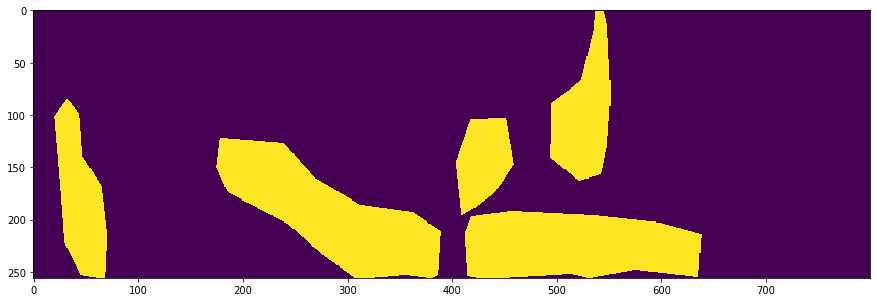
\includegraphics[width = 0.5\textwidth]{images/true_def2.png}}
    \subfloat[Defect 3 Prediction]{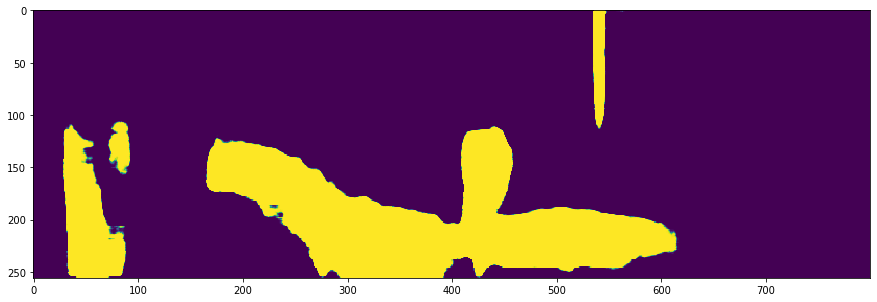
\includegraphics[width = 0.5\textwidth]{images/pred_def2.png}}\\
    \subfloat[Defect 4 Mask]{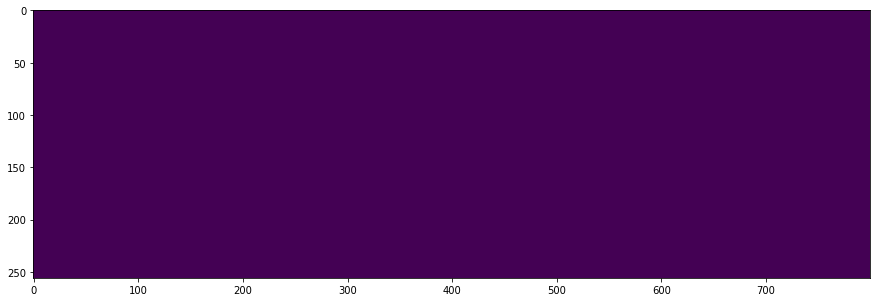
\includegraphics[width = 0.5\textwidth]{images/true_def3.png}}
    \subfloat[Defect 4 Prediction]{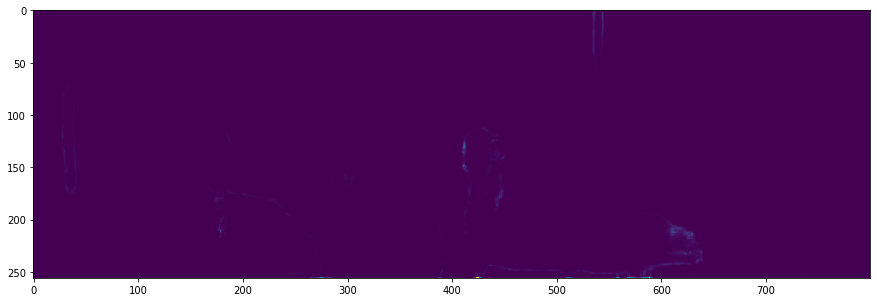
\includegraphics[width = 0.5\textwidth]{images/pred_def3.png}}
    \caption{A visualization of the network's performance in predicting defects.}
    \label{figure:example_steel_prediction}
\end{figure}